% Options for packages loaded elsewhere
\PassOptionsToPackage{unicode}{hyperref}
\PassOptionsToPackage{hyphens}{url}
%
\documentclass[
]{book}
\usepackage{lmodern}
\usepackage{amssymb,amsmath}
\usepackage{ifxetex,ifluatex}
\ifnum 0\ifxetex 1\fi\ifluatex 1\fi=0 % if pdftex
  \usepackage[T1]{fontenc}
  \usepackage[utf8]{inputenc}
  \usepackage{textcomp} % provide euro and other symbols
\else % if luatex or xetex
  \usepackage{unicode-math}
  \defaultfontfeatures{Scale=MatchLowercase}
  \defaultfontfeatures[\rmfamily]{Ligatures=TeX,Scale=1}
\fi
% Use upquote if available, for straight quotes in verbatim environments
\IfFileExists{upquote.sty}{\usepackage{upquote}}{}
\IfFileExists{microtype.sty}{% use microtype if available
  \usepackage[]{microtype}
  \UseMicrotypeSet[protrusion]{basicmath} % disable protrusion for tt fonts
}{}
\makeatletter
\@ifundefined{KOMAClassName}{% if non-KOMA class
  \IfFileExists{parskip.sty}{%
    \usepackage{parskip}
  }{% else
    \setlength{\parindent}{0pt}
    \setlength{\parskip}{6pt plus 2pt minus 1pt}}
}{% if KOMA class
  \KOMAoptions{parskip=half}}
\makeatother
\usepackage{xcolor}
\IfFileExists{xurl.sty}{\usepackage{xurl}}{} % add URL line breaks if available
\IfFileExists{bookmark.sty}{\usepackage{bookmark}}{\usepackage{hyperref}}
\hypersetup{
  pdftitle={DMAC Training Modules},
  pdfauthor={Kyle Roell, Lauren Koval, Julia Rager},
  hidelinks,
  pdfcreator={LaTeX via pandoc}}
\urlstyle{same} % disable monospaced font for URLs
\usepackage{color}
\usepackage{fancyvrb}
\newcommand{\VerbBar}{|}
\newcommand{\VERB}{\Verb[commandchars=\\\{\}]}
\DefineVerbatimEnvironment{Highlighting}{Verbatim}{commandchars=\\\{\}}
% Add ',fontsize=\small' for more characters per line
\usepackage{framed}
\definecolor{shadecolor}{RGB}{248,248,248}
\newenvironment{Shaded}{\begin{snugshade}}{\end{snugshade}}
\newcommand{\AlertTok}[1]{\textcolor[rgb]{0.94,0.16,0.16}{#1}}
\newcommand{\AnnotationTok}[1]{\textcolor[rgb]{0.56,0.35,0.01}{\textbf{\textit{#1}}}}
\newcommand{\AttributeTok}[1]{\textcolor[rgb]{0.77,0.63,0.00}{#1}}
\newcommand{\BaseNTok}[1]{\textcolor[rgb]{0.00,0.00,0.81}{#1}}
\newcommand{\BuiltInTok}[1]{#1}
\newcommand{\CharTok}[1]{\textcolor[rgb]{0.31,0.60,0.02}{#1}}
\newcommand{\CommentTok}[1]{\textcolor[rgb]{0.56,0.35,0.01}{\textit{#1}}}
\newcommand{\CommentVarTok}[1]{\textcolor[rgb]{0.56,0.35,0.01}{\textbf{\textit{#1}}}}
\newcommand{\ConstantTok}[1]{\textcolor[rgb]{0.00,0.00,0.00}{#1}}
\newcommand{\ControlFlowTok}[1]{\textcolor[rgb]{0.13,0.29,0.53}{\textbf{#1}}}
\newcommand{\DataTypeTok}[1]{\textcolor[rgb]{0.13,0.29,0.53}{#1}}
\newcommand{\DecValTok}[1]{\textcolor[rgb]{0.00,0.00,0.81}{#1}}
\newcommand{\DocumentationTok}[1]{\textcolor[rgb]{0.56,0.35,0.01}{\textbf{\textit{#1}}}}
\newcommand{\ErrorTok}[1]{\textcolor[rgb]{0.64,0.00,0.00}{\textbf{#1}}}
\newcommand{\ExtensionTok}[1]{#1}
\newcommand{\FloatTok}[1]{\textcolor[rgb]{0.00,0.00,0.81}{#1}}
\newcommand{\FunctionTok}[1]{\textcolor[rgb]{0.00,0.00,0.00}{#1}}
\newcommand{\ImportTok}[1]{#1}
\newcommand{\InformationTok}[1]{\textcolor[rgb]{0.56,0.35,0.01}{\textbf{\textit{#1}}}}
\newcommand{\KeywordTok}[1]{\textcolor[rgb]{0.13,0.29,0.53}{\textbf{#1}}}
\newcommand{\NormalTok}[1]{#1}
\newcommand{\OperatorTok}[1]{\textcolor[rgb]{0.81,0.36,0.00}{\textbf{#1}}}
\newcommand{\OtherTok}[1]{\textcolor[rgb]{0.56,0.35,0.01}{#1}}
\newcommand{\PreprocessorTok}[1]{\textcolor[rgb]{0.56,0.35,0.01}{\textit{#1}}}
\newcommand{\RegionMarkerTok}[1]{#1}
\newcommand{\SpecialCharTok}[1]{\textcolor[rgb]{0.00,0.00,0.00}{#1}}
\newcommand{\SpecialStringTok}[1]{\textcolor[rgb]{0.31,0.60,0.02}{#1}}
\newcommand{\StringTok}[1]{\textcolor[rgb]{0.31,0.60,0.02}{#1}}
\newcommand{\VariableTok}[1]{\textcolor[rgb]{0.00,0.00,0.00}{#1}}
\newcommand{\VerbatimStringTok}[1]{\textcolor[rgb]{0.31,0.60,0.02}{#1}}
\newcommand{\WarningTok}[1]{\textcolor[rgb]{0.56,0.35,0.01}{\textbf{\textit{#1}}}}
\usepackage{longtable,booktabs}
% Correct order of tables after \paragraph or \subparagraph
\usepackage{etoolbox}
\makeatletter
\patchcmd\longtable{\par}{\if@noskipsec\mbox{}\fi\par}{}{}
\makeatother
% Allow footnotes in longtable head/foot
\IfFileExists{footnotehyper.sty}{\usepackage{footnotehyper}}{\usepackage{footnote}}
\makesavenoteenv{longtable}
\usepackage{graphicx,grffile}
\makeatletter
\def\maxwidth{\ifdim\Gin@nat@width>\linewidth\linewidth\else\Gin@nat@width\fi}
\def\maxheight{\ifdim\Gin@nat@height>\textheight\textheight\else\Gin@nat@height\fi}
\makeatother
% Scale images if necessary, so that they will not overflow the page
% margins by default, and it is still possible to overwrite the defaults
% using explicit options in \includegraphics[width, height, ...]{}
\setkeys{Gin}{width=\maxwidth,height=\maxheight,keepaspectratio}
% Set default figure placement to htbp
\makeatletter
\def\fps@figure{htbp}
\makeatother
\setlength{\emergencystretch}{3em} % prevent overfull lines
\providecommand{\tightlist}{%
  \setlength{\itemsep}{0pt}\setlength{\parskip}{0pt}}
\setcounter{secnumdepth}{5}
\usepackage{booktabs}
\usepackage[]{natbib}
\bibliographystyle{plainnat}

\title{DMAC Training Modules}
\author{Kyle Roell, Lauren Koval, Julia Rager}
\date{2021-06-04}

\begin{document}
\maketitle

{
\setcounter{tocdepth}{1}
\tableofcontents
}
\hypertarget{introduction}{%
\chapter{Introduction}\label{introduction}}

The \href{https://sph.unc.edu/superfund-pages/srp/}{UNC-Superfund Research Program} (SRP) seeks to develop new solutions for reducing exposure to inorganic arsenic and prevent arsenic-induced diabetes through mechanistic and translational research.

The \href{https://sph.unc.edu/superfund-pages/dmac/}{Data Analysis and Management Core} (DMAC) provide the UNC-Superfund Research Program with critical expertise in bioinformatics, statistics, data management and data integration. Our goal is to support the data management, integration, and analysis needs of the researchers to reveal multi-factorial determinants of inorganic arsenic-induced metabolic dysfunction/diabetes.

All code for these modules can be found at the \href{https://github.com/UNCSRP}{UNC-SRP Github Page}.


\includegraphics[width=45.58in]{_book/test1_files/figure-html/SRP_logo}

\hypertarget{intro}{%
\chapter{Setting Up Your R Environment}\label{intro}}

Before learning about data manipulation and statistical methods for analyzing environmental health datasets, we will provide a brief introduction to R, RStudio, and setting up an R environment and simple scripts.

\hypertarget{r-and-rstudio}{%
\section{R and RStudio}\label{r-and-rstudio}}

\href{https://www.r-project.org}{R} is a free, open source programming language for statistical computing and graphics that anyone can download and use. It doesn't require a license and is good for reproducible analyses. There exists a large, diverse collection of packages and very comprehensive documentation.

It is easy to download, install, and setup R. Additionally, \href{https://www.rstudio.com}{RStudio} is an open source integrated development environment for R. RStudio makes programming in R and using R scripts and features more user friendly. R should be downloaded prior to downloading RStudio.

\hypertarget{downloading-r-and-rstudio}{%
\subsection{Downloading R and RStudio}\label{downloading-r-and-rstudio}}

The following is a walkthrough on how to download R and RStudio.

\textbf{1. Navigate to R Website}

\begin{figure}
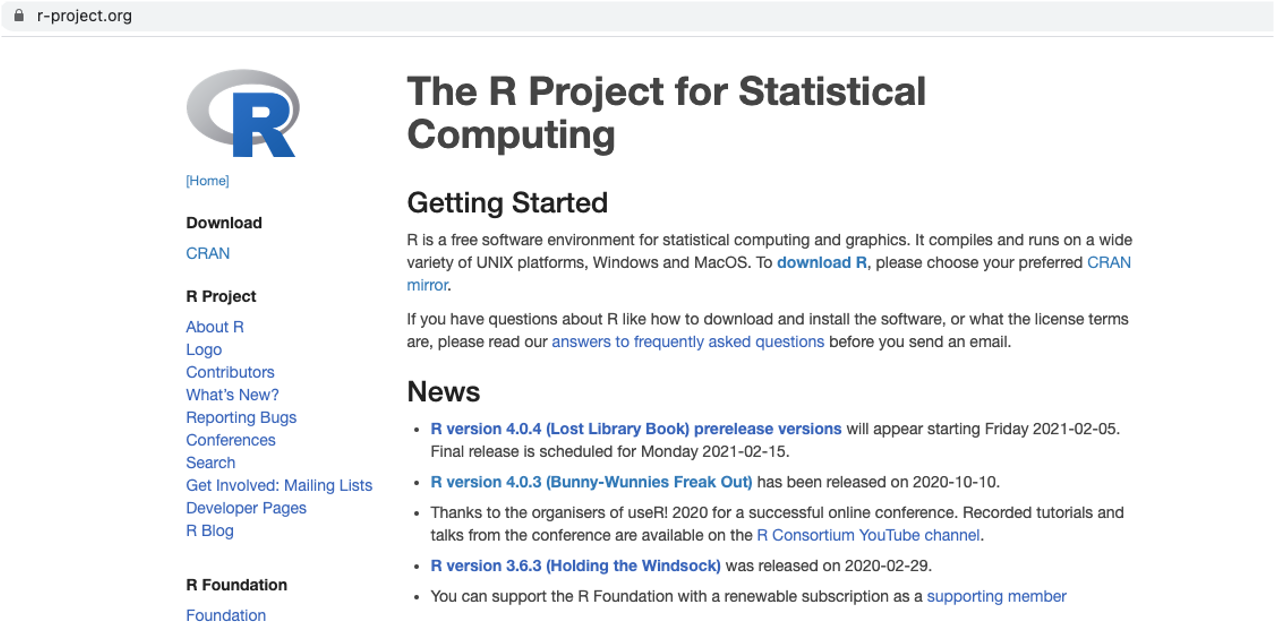
\includegraphics[width=17.71in]{_book/test1_files/figure-html/r_website} \caption{R Website, https://www.r-project.org}\label{fig:website}
\end{figure}

\textbf{2. Select the appropriate CRAN mirror (Duke is fastest if at UNC)}

\begin{figure}
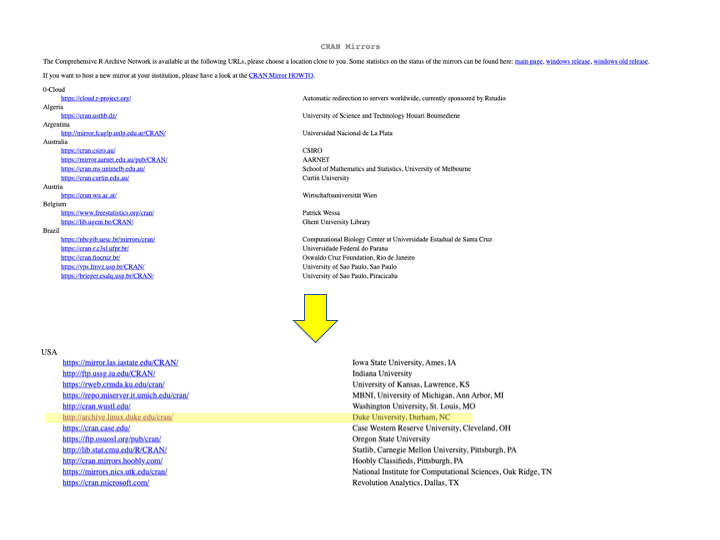
\includegraphics[width=17.85in]{_book/test1_files/figure-html/cran_mirrors} \caption{CRAN Mirror, https://cran.r-project.org/mirrors.html}\label{fig:mirror}
\end{figure}

\textbf{3. Select the appropriate R distribution}

\begin{figure}
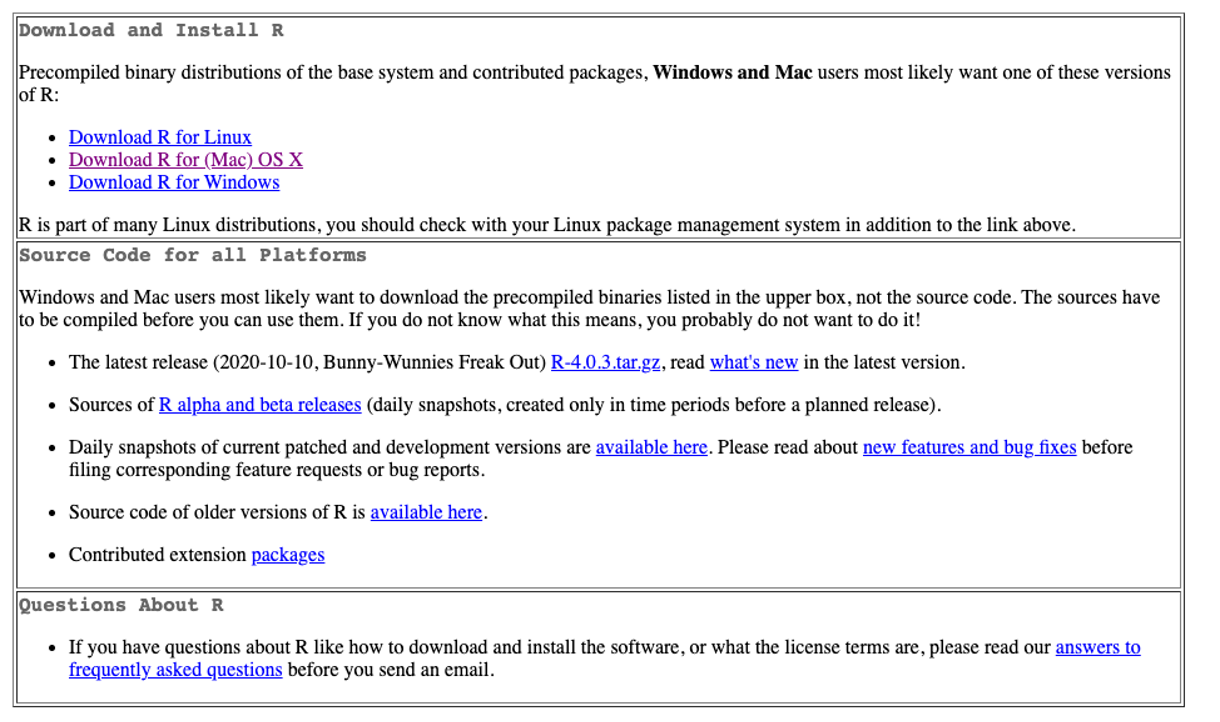
\includegraphics[width=16.94in]{_book/test1_files/figure-html/duke_archive_r} \caption{R Download Link, http://archive.linux.duke.edu/cran/}\label{fig:archive}
\end{figure}

\textbf{4. Download R}

\begin{figure}
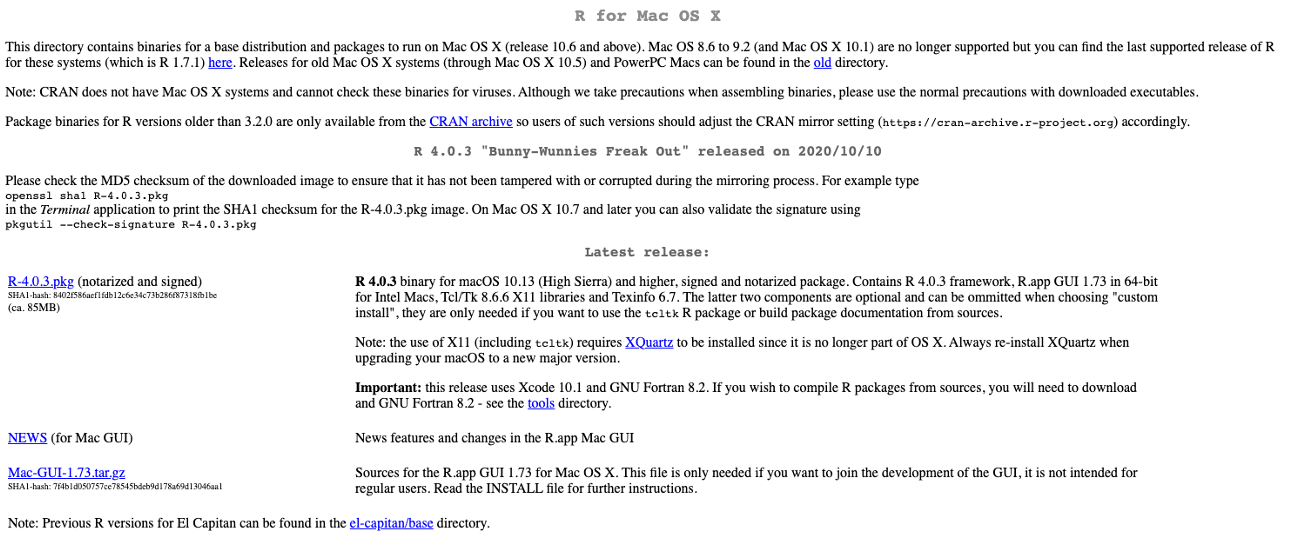
\includegraphics[width=17.93in]{_book/test1_files/figure-html/duke_download_r} \caption{R Download, http://archive.linux.duke.edu/cran/bin/macosx/}\label{fig:download}
\end{figure}

\textbf{5. Navigate to RStudio website and download RStudio (free edition)}

\begin{figure}
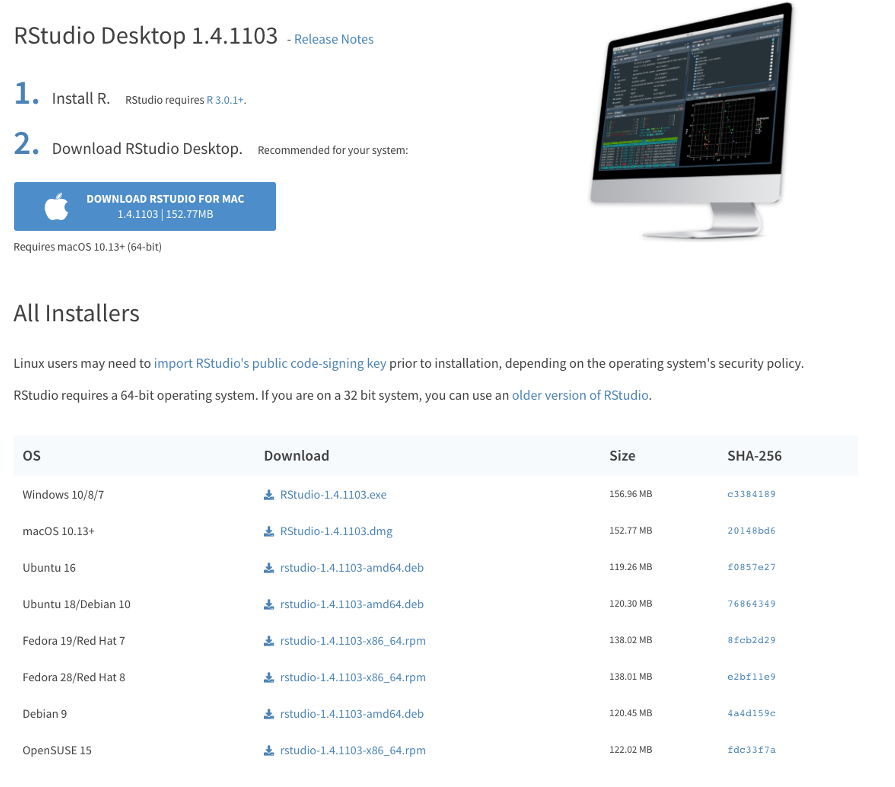
\includegraphics[width=12.43in]{_book/test1_files/figure-html/rstudio} \caption{RStudio Download, https://rstudio.com/products/rstudio/download/}\label{fig:downloadstudio}
\end{figure}

\hypertarget{installing-r-and-rstudio}{%
\subsection{Installing R and RStudio}\label{installing-r-and-rstudio}}

Once R and RStudio have been downloaded, install R first and then RStudio, following the instructions of the installer.

\hypertarget{installing-and-loading-packages}{%
\subsection{Installing and Loading Packages}\label{installing-and-loading-packages}}

Packages in R are units of shareable code that contain functions, data, and documentation on how to use all of these resources. Because R is an open source programming language, packages are constantly being developed and updated. There are many R packages that exist spanning many topics such as graphics and plotting, machine learning, and data manipulation. R packages are often written by R users and submitted to the \href{https://cran.r-project.org}{Comprehensive R Archive Network} (CRAN), or another host such as \href{https://www.bioconductor.org}{BioConductor} or \href{https://github.com}{GitHub}.

Packages can be installed from the host, but need to be loaded into the workspace. Most of the time, you do not need to download anything from a website. Instead, you can install packages through running code in R or RStudio.

\begin{Shaded}
\begin{Highlighting}[]
\KeywordTok{install.packages}\NormalTok{(}\StringTok{"ggplot2"}\NormalTok{, }\DataTypeTok{repos =} \StringTok{"https://cran.rstudio.com"}\NormalTok{)}
\end{Highlighting}
\end{Shaded}

Once a package is installed, it needs to be loaded using the \emph{library} function or explicitly referenced to use functions or datasets from that package.

\begin{Shaded}
\begin{Highlighting}[]
\KeywordTok{library}\NormalTok{(ggplot2)}
\end{Highlighting}
\end{Shaded}

\hypertarget{scripting-basics}{%
\section{Scripting Basics}\label{scripting-basics}}

Before demonstrating the basics of writing R code and scripts, it is worth noting that a function can be queried in RStudio by typing a question mark before the name of the function (e.g.~\emph{?install.packages}). This will bring up documentation in the viewer window. Additionally, RStudio will autofill function names, variable names, etc. by pressing tab while typing. If multiple matches are found, RStudio will provide you with a drop down list to select from, which may be useful when searching through newly installed packages or trying to quickly type variable names in an R script.

R also allows for scripts to contain non-code elements, called comments, that will not be run or interpreted. To make a comment, simply use a \# followed by the comment. A \# only comments out a single line of code, i.e.~only that line will not be run. Comments are useful to help make code more interpretable for others or to add reminders of what and why parts of code may have been written.

\begin{Shaded}
\begin{Highlighting}[]
\CommentTok{# This is an R comment!}

\CommentTok{# Loading ggplot2 package}
\KeywordTok{library}\NormalTok{(ggplot2)}
\end{Highlighting}
\end{Shaded}

\hypertarget{setting-working-directory}{%
\subsection{Setting Working Directory}\label{setting-working-directory}}

When working in R, it can be helpful to set the working directory to a local directory where data are located or output files will be saved. The current working directory can also be displayed.

\begin{Shaded}
\begin{Highlighting}[]
\CommentTok{# Show current working directory}
\KeywordTok{getwd}\NormalTok{()}
\end{Highlighting}
\end{Shaded}

\begin{verbatim}
## [1] "/Users/kroell/Documents/IEHS/UNC-SRP/test1"
\end{verbatim}

\begin{Shaded}
\begin{Highlighting}[]
\CommentTok{# Set working directory}
\KeywordTok{setwd}\NormalTok{(}\StringTok{"~/Documents/UNCSRP/Data/"}\NormalTok{)}
\end{Highlighting}
\end{Shaded}

\hypertarget{importing-and-exporting-files}{%
\subsection{Importing and Exporting Files}\label{importing-and-exporting-files}}

After setting the working directory, importing and exporting files can be done using various functions based on the type of file being read or written. Often, it is easiest to import data into R that are in a comma separated values, comma delimited, (CSV) file or tab delimited file. Other datatypes such as SAS data files, large csv files, etc. may require different functions to be more efficienlty read in and some of these file formats will be discussed in future modules.

\begin{Shaded}
\begin{Highlighting}[]
\CommentTok{# Read in CSV data}
\NormalTok{csv.dataset =}\StringTok{ }\KeywordTok{read.csv}\NormalTok{(}\DataTypeTok{file=}\StringTok{"~/Documents/UNCSRP/Data/example_data.csv"}\NormalTok{)}

\CommentTok{# Read in tab delimited data}
\NormalTok{tab.dataset =}\StringTok{ }\KeywordTok{read.table}\NormalTok{(}\DataTypeTok{file=}\StringTok{"~/Documents/UNCSRP/Data/example_data.txt"}\NormalTok{)}
\end{Highlighting}
\end{Shaded}

There are many ways to export data in R. Data can be written out into a CSV file, tab delimited file, RData file, etc. There are also many functions within packages that write out specific datasets generated by that package.

\begin{Shaded}
\begin{Highlighting}[]
\CommentTok{# Write out to a CSV file}
\KeywordTok{write.csv}\NormalTok{(csv.output, }\DataTypeTok{file=}\StringTok{"~/Documents/UNCSRP/Output/csv_output.csv"}\NormalTok{)}

\CommentTok{# Write out to a tab delimited file}
\KeywordTok{write.table}\NormalTok{(tab.output, }\DataTypeTok{file=}\StringTok{"~/Documents/UNCSRP/Output/tsv_output.txt"}\NormalTok{, }\DataTypeTok{sep=}\StringTok{"}\CharTok{\textbackslash{}t}\StringTok{"}\NormalTok{)}
\end{Highlighting}
\end{Shaded}

R also allows objects to be saved in RData files. These files can be read into R, as well, and will load the object into the current workspace. Entire workspaces are also able to be saved.

\begin{Shaded}
\begin{Highlighting}[]
\CommentTok{# Read in saved single R data object}
\NormalTok{r.obj =}\StringTok{ }\KeywordTok{readRDS}\NormalTok{(}\DataTypeTok{file=}\StringTok{"~/Documents/UNCSRP/Data/data.rds"}\NormalTok{)}

\CommentTok{# Write single R object to file}
\KeywordTok{saveRDS}\NormalTok{(object, }\DataTypeTok{file=}\StringTok{"~/Documents/UNCSRP/Output/single_object.rds"}\NormalTok{)}

\CommentTok{# Read in multiple saved R objects}
\KeywordTok{load}\NormalTok{(}\DataTypeTok{file=}\StringTok{"~/Documents/UNCSRP/Data/multiple_data.RData"}\NormalTok{)}

\CommentTok{# Save multiple R objects}
\KeywordTok{save}\NormalTok{(object1, object2, }\DataTypeTok{file=}\StringTok{"~/Documents/UNCSRP/Output/multiple_objects.RData"}\NormalTok{)}

\CommentTok{# Save entire workspace}
\KeywordTok{save.image}\NormalTok{(}\DataTypeTok{file=}\StringTok{"~/Documents/UNCSRP/Output/entire_workspace.RData"}\NormalTok{)}

\CommentTok{# Load entire workspace}
\KeywordTok{load}\NormalTok{(}\DataTypeTok{file=}\StringTok{"~/Documents/UNCSRP/Data/entire_workspace.RData"}\NormalTok{)}
\end{Highlighting}
\end{Shaded}

\hypertarget{viewing-data}{%
\subsection{Viewing Data}\label{viewing-data}}

After data has been loaded into R, or created within R, it is good to inspect it. Datasets can be viewed in their entirety or subset to quickly look at part of the data.

\begin{Shaded}
\begin{Highlighting}[]
\CommentTok{# View first 5 rows of the previously loaded dataset}
\NormalTok{csv.dataset[}\DecValTok{1}\OperatorTok{:}\DecValTok{5}\NormalTok{,]}
\end{Highlighting}
\end{Shaded}

\begin{verbatim}
##    Sample Var1 Var2 Var3
## 1 sample1    1    2    1
## 2 sample2    2    4    4
## 3 sample3    3    6    9
## 4 sample4    4    8   16
## 5 sample5    5   10   25
\end{verbatim}

\begin{Shaded}
\begin{Highlighting}[]
\CommentTok{# View the entire dataset in RStudio}
\KeywordTok{View}\NormalTok{(csv.dataset)}
\end{Highlighting}
\end{Shaded}

\hypertarget{dataorg}{%
\chapter{The Basics for Data Organization}\label{dataorg}}

\hypertarget{basic-data-manipulation}{%
\section{Basic Data Manipulation}\label{basic-data-manipulation}}

\hypertarget{merging}{%
\subsection{Merging}\label{merging}}

\hypertarget{merging-processed-data-with-metadata-file}{%
\subsection{Merging processed data with metadata file?}\label{merging-processed-data-with-metadata-file}}

\hypertarget{cast}{%
\subsection{Cast}\label{cast}}

\hypertarget{melt}{%
\subsection{Melt}\label{melt}}

\hypertarget{filtering-subsetting}{%
\subsection{Filtering \& subsetting}\label{filtering-subsetting}}

\hypertarget{tidyverse-stuff-pivots}{%
\subsection{Tidyverse stuff (pivots)}\label{tidyverse-stuff-pivots}}

\hypertarget{finding-and-visualizing-data-trends}{%
\chapter{Finding and Visualizing Data Trends}\label{finding-and-visualizing-data-trends}}

\hypertarget{heat-maps}{%
\section{Heat maps}\label{heat-maps}}

\hypertarget{pheatmap}{%
\subsection{pheatmap}\label{pheatmap}}

\hypertarget{heatmap2}{%
\subsection{heatmap2}\label{heatmap2}}

\hypertarget{superheat}{%
\subsection{superheat}\label{superheat}}

\hypertarget{clustering}{%
\section{Clustering}\label{clustering}}

Examples with genomics: Rager et al.~2014

\hypertarget{hierarchical}{%
\subsection{Hierarchical}\label{hierarchical}}

\hypertarget{k-means}{%
\subsection{K-means}\label{k-means}}

\hypertarget{data-reduction-pca}{%
\section{Data reduction (PCA)}\label{data-reduction-pca}}

\hypertarget{visualize-pca-plot}{%
\subsection{Visualize PCA Plot}\label{visualize-pca-plot}}

\hypertarget{identify-of-variance-captured}{%
\subsection{Identify \% of variance captured}\label{identify-of-variance-captured}}

\hypertarget{basic-statistical-tests-and-visualizations-of-data}{%
\section{Basic Statistical Tests and Visualizations of Data}\label{basic-statistical-tests-and-visualizations-of-data}}

Need an example dataset -- maybe ELGAN shuffled/deidentified, with made-up environmental exposure column?

\hypertarget{normality}{%
\subsection{Normality}\label{normality}}

Kruskal wallis? The other one that I always forget? Shapiro wilks? - histogram

\hypertarget{t-tests-column-charts}{%
\subsection{T-tests -- column charts}\label{t-tests-column-charts}}

\hypertarget{regression-linear-regression-and-logistic-regression}{%
\subsection{Regression: linear regression and logistic regression}\label{regression-linear-regression-and-logistic-regression}}

\hypertarget{anova-delicate-commentary}{%
\subsection{ANOVA + delicate commentary}\label{anova-delicate-commentary}}

\hypertarget{chi-squared-test-box-plots}{%
\subsection{Chi-squared test -- box plots}\label{chi-squared-test-box-plots}}

\hypertarget{fishers-exact-test}{%
\subsection{Fisher's exact test}\label{fishers-exact-test}}

\hypertarget{multi-omics-analyses-for-environmental-health}{%
\chapter{Multi-Omics Analyses for Environmental Health}\label{multi-omics-analyses-for-environmental-health}}

\hypertarget{exposomics}{%
\section{Exposomics}\label{exposomics}}

\hypertarget{placenta-exposome}{%
\subsection{Placenta Exposome}\label{placenta-exposome}}

about to be submitted to EI
Dust NTA data

\hypertarget{transcriptomics}{%
\section{Transcriptomics}\label{transcriptomics}}

\hypertarget{deseq2-rnaseq}{%
\subsection{DESeq2 / RNAseq}\label{deseq2-rnaseq}}

Wildfire dataset, available through GEO

\hypertarget{genome-wide-microrna}{%
\section{Genome-wide MicroRNA}\label{genome-wide-microrna}}

Rager et al.~2014 miRNAs

\hypertarget{genome-wide-dna-methylation}{%
\section{Genome-wide DNA Methylation}\label{genome-wide-dna-methylation}}

\hypertarget{illumina-array-data}{%
\subsection{Illumina array data}\label{illumina-array-data}}

\begin{verbatim}
https://www.ncbi.nlm.nih.gov/geo/query/acc.cgi?acc=GSE58499
https://www.ncbi.nlm.nih.gov/geo/query/acc.cgi?acc=GSE28368
\end{verbatim}

\hypertarget{proteomics}{%
\section{Proteomics}\label{proteomics}}

\begin{verbatim}
Bailey et al arsenic dataset maybe?
\end{verbatim}

\hypertarget{mixtures-analyses-for-environmental-health}{%
\chapter{Mixtures Analyses for Environmental Health}\label{mixtures-analyses-for-environmental-health}}

\hypertarget{sufficient-similarity}{%
\section{Sufficient Similarity}\label{sufficient-similarity}}

Botanicals example with chemistry and tox profiling -- Julia has dataset

\hypertarget{mixtures-modeling-through-qgcomp}{%
\section{Mixtures Modeling through qgcomp}\label{mixtures-modeling-through-qgcomp}}

Could use published wildfire analysis here (Rager et al.~2021, STOTEN), or online example provide through Alex Keil's studies

\hypertarget{environmental-health-databases}{%
\chapter{Environmental Health Databases}\label{environmental-health-databases}}

\hypertarget{comparative-toxicogenomics-database-ctd}{%
\section{Comparative Toxicogenomics Database (CTD)}\label{comparative-toxicogenomics-database-ctd}}

\hypertarget{gene-expression-omnibus-geo}{%
\section{Gene Expression Omnibus (GEO)}\label{gene-expression-omnibus-geo}}

\hypertarget{nhanes}{%
\section{NHANES}\label{nhanes}}

\end{document}
